\documentclass{standalone}%scrreprt
\usepackage{pgfplots}
\usepackage{tikz}
\usepackage{tikz-network}
\usepackage{amsmath}
\usepackage{verbatim}
\usepackage[dvipsnames]{xcolor}

\usetikzlibrary{arrows,shapes,backgrounds,positioning}

\begin{comment}
Multilayer example following tikz-networks package
\end{comment}
\usetikzlibrary{3d}

\begin{document}

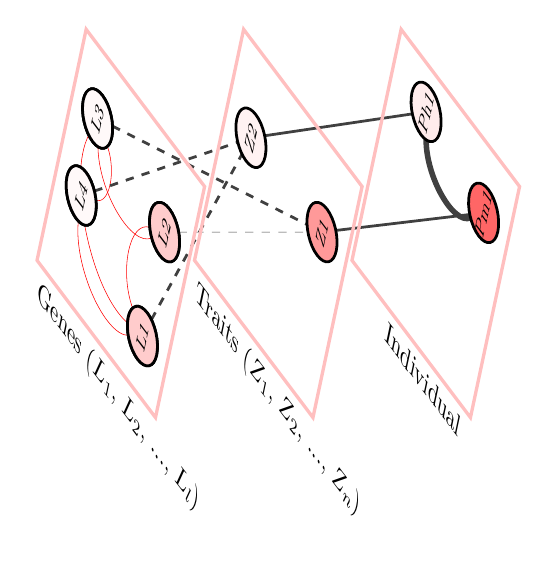
\begin{tikzpicture}[multilayer=3d,rotate=90]
%\begin{tikzpicture}[multilayer=3d]
\begin{Layer}[layer=1]
\draw[very thick,pink!100] (-.5,-.5) rectangle (2.5,2);
\node at (-.5,2)[below right,rotate=270]{Genes ($L_{1}$, $L_{2}$, ..., $L_{l}$)};
\end{Layer}
\Vertex[x=0.15,IdAsLabel,layer=1,color=red!20]{L1}
\Vertex[x=1.5,IdAsLabel,layer=1,color=red!20]{L2}
\Vertex[x=1.75,y=1.5,IdAsLabel,layer=1,color=pink!10]{L3}
\Vertex[x=0.75,y=1.5,IdAsLabel,layer=1,color=pink!10]{L4}

%\Vertex[x=-0.5,IdAsLabel,size=0.3,layer=1,color=red!20]{E}
%\Vertex[x=-0.35,IdAsLabel,size=0.3,layer=1,color=red!20]{F}
%\Vertex[x=-0.25,y=1.5,size=0.3,IdAsLabel,layer=1,color=pink!10]{G}
%\Vertex[x=0.15,y=1.5,size=0.3,IdAsLabel,layer=1,color=pink!10]{H}

\SetLayerDistance{-2}

\begin{Layer}[layer=2]
\draw[very thick,pink!100] (-.5,-.5) rectangle (2.5,2);
\node at (-.5,2)[below right,rotate=270]{Traits ($Z_{1}$, $Z_{2}$, ..., $Z_{n}$)};
\end{Layer}
\Vertex[x=0.15,IdAsLabel,layer=1,color=red!20]{L1}
\Vertex[x=1.5,IdAsLabel,layer=1,color=red!20]{L2}
\Vertex[x=1.75,y=1.5,IdAsLabel,layer=1,color=pink!10]{L3}
\Vertex[x=0.75,y=1.5,IdAsLabel,layer=1,color=pink!10]{L4}

\SetLayerDistance{-2}

\begin{Layer}[layer=3]
\draw[very thick,pink!100] (-.5,-.5) rectangle (2.5,2);
\node at (-.5,-.5)[below left,rotate=270]{Individual};
\end{Layer}
\Vertex[x=1.5,IdAsLabel,layer=2,color=red!40]{Z1}
\Vertex[x=1.5,y=1.5,IdAsLabel,layer=2,color=pink!20]{Z2}

%\SetLayerDistance{-2}

%\begin{Layer}[layer=4]
%\draw[very thick,pink!60] (-.5,-.5) rectangle (2.5,2);
%\node at (-.5,-.5)[below left,rotate=270]{Population};
%\end{Layer}
\Vertex[x=1.75,IdAsLabel,layer=3,color=red!60]{Pm1}
\Vertex[x=2,y=1.3,IdAsLabel,layer=3,color=pink!30]{Ph1}

%\SetLayerDistance{-2}

%\begin{Layer}[layer=5]
%\draw[very thick,pink!80] (-.5,-.5) rectangle (2.5,2);
%\node at (-.5,-.5)[below left,rotate=270]{Species};
%\end{Layer}
%\Vertex[x=0.02,IdAsLabel,size=0.7,layer=4,color=red!80]{M}
%\Vertex[x=2,y=1.3,IdAsLabel,size=0.7,layer=4,color=pink!50]{H}

%\SetLayerDistance{-2}

%\begin{Layer}[layer=6]
%\draw[very thick,black!90] (-.5,-.5) rectangle (2.5,2);
%\Plane[x=-.5,y=-.5,width=2.75,height=2.75,style={inner
%color=red,outer color=pink!80}]
%\node at (-.5,-.5)[below left,rotate=270]{Biodiversity};
%\node at (-.5,-.5)[below right]{{\bf Eco-evolutionary dynamics}};
%\end{Layer}
%\Vertex[x=1.8,y=1.75,IdAsLabel,size=0.7,layer=6,color=red!30]{SH}
%\Vertex[x=1,y=1.5,IdAsLabel,size=0.7,layer=6,color=red!70]{SM}

%\SetLayerDistance{-2}

%\begin{Layer}[layer=7]
%\draw[very thick,black!90] (-.5,-.5) rectangle (2.5,2);
%\Plane[x=-.5,y=-.5,width=2.75,height=2.75,style={inner
%color=brown,outer color=brown!60}]
%\node at (-.5,-.5)[below left,rotate=270]{Functions};
%\node at (-.5,-.5)[below right]{{\bf Eco-evolutionary dynamics}};
%\end{Layer}
%\Vertex[x=1.8,y=1.75,IdAsLabel,size=0.7,layer=7,color=brown!30]{FH}
%\Vertex[x=1,y=1.5,IdAsLabel,size=0.7,layer=7,color=brown!70]{FM}


%\begin{Layer}[layer=7]
%\draw[very thick,black!90] (-.5,-.5) rectangle (2.5,2);
%\Plane[x=-.5,y=-.5,width=2.75,height=2.75,style={inner
%color=brown,outer color=pink!40}]
%\node at (-.5,-.5)[below left,rotate=270]{Functions};
%\node at (-.5,-.5)[below right]{{\bf Eco-evolutionary dynamics}};
%\Vertex[x=1.8,y=1.75,IdAsLabel,size=0.7,layer=7,color=brown!30]{F1}
%\Vertex[x=1,y=1.5,IdAsLabel,size=0.7,layer=7,color=brown!70]{F2}
%\end{Layer}


%Environmental layer

%\begin{Layer}[layer=7]
%\draw[very thick,black!90] (-.5,-.5) rectangle (2.5,2);
%\Plane[x=-.5,y=-.5,width=2.75,height=2.75,style={inner
%color=brown,outer color=pink!40}]
%\node at (-.5,-.5)[below left,rotate=270]{Functions};
%\node at (-.5,-.5)[below right]{{\bf Eco-evolutionary dynamics}};
%\end{Layer}

%\Vertex[x=0.2,IdAsLabel,size=0.5,layer=5,color=red]{S1m}
%\Vertex[x=0.7,IdAsLabel,size=0.5,layer=5,color=red]{S2m}
%\Vertex[y=1.1,IdAsLabel,size=0.5,layer=5,color=red]{S3m}
%\Vertex[y=1.8,IdAsLabel,size=0.6,layer=5,color=red]{S4m}

%\Vertex[x=1,y=1.7,IdAsLabel,size=0.4,layer=5,color=pink!40]{S1h}
%\Vertex[x=0.75,y=0.8,IdAsLabel,size=0.4,layer=5,color=pink!40]{S2h}
%\Vertex[x=1.1,y=1,IdAsLabel,size=0.4,layer=5,color=pink!40]{S3h}
%\Vertex[x=1.8,y=1.2,IdAsLabel,size=0.5,layer=5,color=pink!40]{S4h}

\Edge[lw=0.2,bend=60,color=red](L1)(L2)
\Edge[lw=0.2,bend=60,color=red](L2)(L3)
\Edge[lw=0.2,bend=60,color=red](L3)(L4)
\Edge[lw=0.2,bend=60,color=red](L1)(L3)
\Edge[lw=0.2,bend=60,color=red](L1)(L4)

\Edge[lw=0.2,style=dashed](L2)(Z1)
\Edge[lw=1,style=dashed](L1)(Z2)
%\Edge[lw=2,bend=60](H1)(M1)
\Edge[lw=1,style=dashed](L3)(Z1)
\Edge[lw=1,style=dashed](L4)(Z2)
\Edge[lw=1](Z1)(Pm1)
\Edge[lw=1](Z2)(Ph1)
\Edge[lw=2,bend=60](Pm1)(Ph1)

%\Edge[lw=2](Pm1)(M)
%\Edge[lw=2](Ph1)(H)
%\Edge[lw=2,bend=60](H)(M)

%\Edge[lw=2](SM)(S1m)
%\Edge[lw=2](SM)(S2m)
%\Edge[lw=2](SM)(S3m)
%\Edge[lw=2](SM)(S4m)

%\Edge[lw=0.2,bend=60](S1m)(S2m)
%\Edge[lw=0.2,bend=60](S1m)(S3m)
%\Edge[lw=0.2,bend=60](S1m)(S4m)
%\Edge[lw=0.2,bend=60](S2m)(S3m)
%\Edge[lw=0.2,bend=60](S2m)(S4m)
%\Edge[lw=0.2,bend=60](S3m)(S4m)

%\Edge[lw=2](M)(S1m)
%\Edge[lw=2](M)(S2m)
%\Edge[lw=2](M)(S3m)
%\Edge[lw=2](M)(S4m)

%\Edge[lw=0.2,bend=60](S1h)(S2h)
%\Edge[lw=0.2,bend=60](S1h)(S3h)
%\Edge[lw=0.2,bend=60](S1h)(S4h)
%Edge[lw=0.2,bend=60](S2h)(S3h)
%\Edge[lw=0.2,bend=60](S2h)(S4h)
%\Edge[lw=0.2,bend=60](S3h)(S4h)

%\Edge[lw=2](H)(S1h)
%\Edge[lw=2](H)(S2h)
%\Edge[lw=2](H)(S3h)
%\Edge[lw=2](H)(S4h)

%\Edge[lw=2](SH)(S1h)
%\Edge[lw=2](SH)(S2h)
%\Edge[lw=2](SH)(S3h)
%\Edge[lw=2](SH)(S4h)

%\Edge[lw=2](SH)(FH)
%\Edge[lw=2](SM)(FM)



%\Edge[lw=0.2,style=dashed,bend=10(S1m)(S2m)
%\Edge[lw=0.2,bend=30](S2m)(S3m)


%---------------------------------

\begin{comment}
%Governance-Exploitation-Recovery-Sustainability dynamics
\SetLayerDistance{-1.27}

\begin{Layer}[layer=6]
\draw[very thick,blue!20] (-.5,-.5) rectangle (2.5,2);
\node at (-.5,-.5)[below left,rotate=270]{Governance};
\end{Layer}
\Vertex[x=0.35,y=1.15,IdAsLabel,size=0.8,layer=6,color=blue!10]{G1}
\Vertex[x=1.5,y=1.15,IdAsLabel,size=0.8,layer=6,color=blue!10]{G2}
\Edge[lw=0.2,style=dashed](M)(G1)
\Edge[lw=0.2,style=dashed](H)(G1)
\Edge[lw=0.2,style=dashed](M)(G2)
\Edge[lw=0.2,style=dashed](H)(G2)


\SetLayerDistance{-1.15}

\begin{Layer}[layer=7]
\draw[very thick,blue!40] (-.5,-.5) rectangle (2.5,2);
\node at (-.5,-.5)[below left,rotate=270]{Exploitation};
\end{Layer}
\Vertex[x=0.35,y=1,IdAsLabel,size=0.6,layer=7,color=blue!30]{E1}
\Vertex[x=1.5,y=1,IdAsLabel,size=0.6,layer=7,color=blue!30]{E2}
\Edge[lw=0.2,style=dashed](G1)(E1)
\Edge[lw=0.2,style=dashed](G1)(E2)
\Edge[lw=0.2,style=dashed](G2)(E1)
\Edge[lw=0.2,style=dashed](G2)(E2)

\SetLayerDistance{-1.1}

\begin{Layer}[layer=8]
\draw[very thick,blue!60] (-.5,-.5) rectangle (2.5,2);
\node at (-.5,-.5)[below left,rotate=270]{Recovery};
\end{Layer}
\Vertex[x=0.75,y=1.2,IdAsLabel,size=0.5,layer=8,color=blue!50]{R1}
\Vertex[x=1.55,y=1.2,IdAsLabel,size=0.5,layer=8,color=blue!50]{R2}
\Edge[lw=0.2,style=dashed](E1)(R1)
\Edge[lw=0.2,style=dashed](E1)(R2)
\Edge[lw=0.2,style=dashed](E2)(R1)
\Edge[lw=0.2,style=dashed](E2)(R2)

\SetLayerDistance{-1.125}

\begin{Layer}[layer=9]
\Plane[x=-.5,y=-.5,width=2.75,height=2.75,style={inner
color=white,outer color=blue!40}]
%\draw[very thick,blue!90] (-.5,-.5) rectangle (2.5,2);
\node at (-.5,-.5)[above left]{};
\node at (-.5,-.5)[below right]{{\bf Sustainability}};
\end{Layer}
\Vertex[x=0.75,y=1.2,IdAsLabel,size=0.75,layer=9,color=blue!10]{S1}
\Vertex[x=1.55,y=1.2,IdAsLabel,size=0.75,layer=9,color=blue!50]{S2}
\Edge[lw=0.2,style=dashed](R1)(S1)
\Edge[lw=0.2,style=dashed](R1)(S2)
\Edge[lw=0.2,style=dashed](R2)(S1)
\Edge[lw=0.2,style=dashed](R2)(S2)

%\Edge[lw=0.2,bend=60](A)(B)
%\Edge[lw=0.2,style=dashed](B)(1)
%\Edge[lw=0.2,style=dashed](1)(P1)
%\Edge[lw=0.2,style=dashed](P1)(S1)

%Software engineering: Renku
%\SetLayerDistance{-1.22}

\begin{Layer}[layer=10]
\draw[very thick,brown!60] (-.5,-.5) rectangle (2.5,2);
\node at (-.5,-.5)[below left,rotate=270]{Replicability};
\end{Layer}
\Vertex[x=0.75,y=1.2,IdAsLabel,size=0.5,layer=10,color=brown!50]{Re1}
\Vertex[x=1.55,y=1.2,IdAsLabel,size=0.5,layer=10,color=brown!50]{Re2}
\Edge[lw=0.2,style=dashed](S1)(Re1)
\Edge[lw=0.2,style=dashed](S1)(Re2)
\Edge[lw=0.2,style=dashed](S2)(Re1)
\Edge[lw=0.2,style=dashed](S2)(Re2)

\SetLayerDistance{-1.18}

\begin{Layer}[layer=11]
\Plane[x=-.5,y=-.5,width=2.75,height=2.75,style={inner
color=white,outer color=brown!40}]
\draw[very thick,blue!90] (-.5,-.5) rectangle (2.5,2);
\node at (-.5,-.5)[below left,rotate=270]{Reproducibility};
\node at (-.5,-.5)[below right]{{\bf Software Engineering}};
\end{Layer}
\Vertex[x=0.75,y=1.2,IdAsLabel,size=0.95,layer=11,color=brown!20]{Rr1}
\Vertex[x=1.55,y=0.2,IdAsLabel,size=0.95,layer=11,color=brown!50]{Rr2}
\Edge[lw=0.2,style=dashed](Re1)(Rr1)
Edge[lw=0.2,style=dashed](Re1)(Rr2)
\Edge[lw=0.2,style=dashed](Re2)(Rr1)
\Edge[lw=0.2,style=dashed](Re2)(Rr2)
\end{comment}

\end{tikzpicture}
%\end{equation}
\end{document}




